\setlength{\parindent}{2em}

\section{基本原理}

\section{发展现状}

\subsection{应用}
\subsubsection{引言}

\subsubsection{原理}
\begin{figure}[ht]
	\centering
	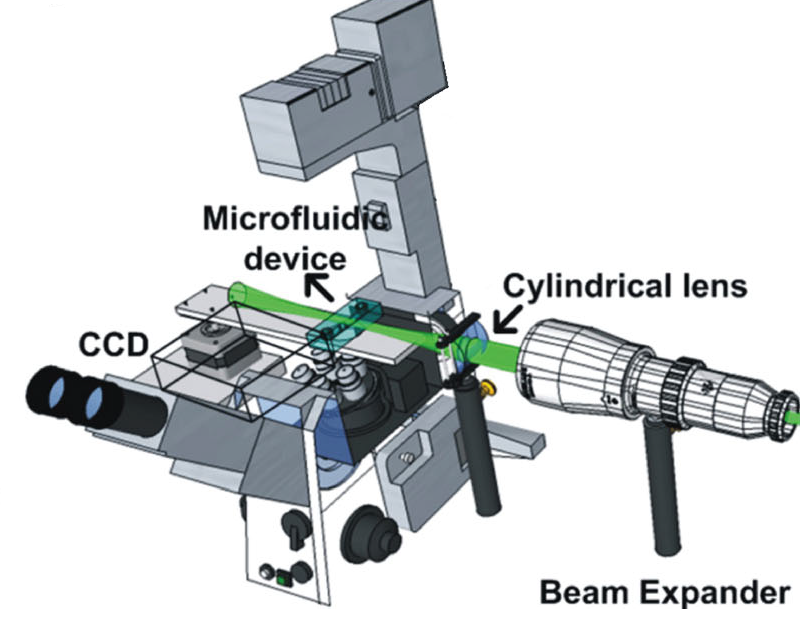
\includegraphics[height=0.7\textwidth]{zhutoujing.png}
	\caption{激光层照荧光显微镜原理结构图\cite{Pampaloni2015Light}}
	\label{fig:4}
\end{figure}
如图\ref{fig:4}

\section{发展现状及前景展望}

\section{仿真计算}
\subsection{题目}
\subsection{计算原理}
\begin{itemize}
	\item 1.点
	\item 2.平
\end{itemize}
\subsection{计算代码}
\subsubsection{生成圆形小孔代码}
\begin{lstlisting}
close all;
clear all;
clc;

N=1024;
z=zeros(N);
[x,y]=meshgrid(1:N);
z((x-N/2).^2+(y-N/2).^2<=(N/4)^2)=1;
imagesc(z);
colormap(gray);
axis square;
axis off;

imwrite(uint8(z),'hahaha.png');
\end{lstlisting}



\subsection{总结分析}
